\chapter{Approach And Methods} % Chapter title

\label{chapter:approach_and_methods} % For referencing the chapter elsewhere, use \ref{chapter:computational_neuro} 

%----------------------------------------------------------------------------------------

\todo{•articipants
(&/oder
Materialen)
Design
Vorgehensweise
z.B. Probanden (Rekrutierung, Anzahl, Beschreibung),
Texte/ Fallstudiendetails, andere Materialen
z.B. Fallstudie, Experiment, Umfrage, strukturierte/halb
strukturierte Interviews etc.
Untersuchte Variablen/Faktoren (abhängige und
unabhängige)
Prozedere (z.B. Verlauf der Umfrage/Experiment, Grafik)
Analyse}
\section{Quantum Basics}
Quantum circuit use qubits instead of classical bits\cite{}. Whilst bits are limited to 0 and 1, qubits can have any state in the range $[0,1]$\cite{}. This cannot be directly measured – once a measurement takes place, the value collapses with a certain probability to either 0 or 1. What can be done is measure the same circuit multiple times. This results in a collection of measurements that resembles the probability of the result taking place. These probabilities can be manipulated using quantum gates of varying functionality.

When parameterizing quantum gates, it is important to note that a rotation takes place. These rotations manipulate the probability of measuring a certain state in the qubit. This can be used to change probabilities according to behaviour defined by us.


\section{Multiple Query Optimization}

\subsection{Data acquisition}
\label{chapter:mqp_data_acquisition}

The problem itself consists of a combination of costs $c$ and savings $s$. These values are basic integer numbers, which for any cost $c$ is in range [1,$x$] and for any saving $s$ in range [$y$,0]. As shown in chapter \ref{chapter:theoretical_fundamentals}, there can be $n$ queries at any given time, each of which has $n_i$ plans. These allow for multiple combinations, which by themselves define the problem space to traverse. To begin with, the problem generator from Fankhauser et al.\cite{fankhauser_multiple_2021} is used to generate a basic problem space consisting of 2 queries, each with 2 plans, as seen in figure \ref{figure:2d_problem_data}.

\begin{figure}[!h]
    \centering
    \begin{minted}{python}
        (2,
          [23, 47, 25, 11],
          {(0, 2): -6,
           (0, 3): -4,
           (1, 2): -13,
           (1, 3): -6})
    \end{minted}
    \caption{This is an automatically generated problem. The first number tells us how many queries there are. In this example, all queries have two plans. The second array containts the cost of running each plan. The third segment is a dictionary where the key symbolizes which plans are combined, and the value of the savings that can be had.}
    \label{figure:2d_problem_data}
\end{figure}

To facilitate the visualization of the problem, they will be numbered from $\mathcal{P}_0$ up to $\mathcal{P}_n$. For example \ref{figure:2d_problem_data}, this would mean that query 1 has plans $\mathcal{P}_0$ and $\mathcal{P}_1$, and query 2 $\mathcal{P}_2$ and $\mathcal{P}_3$, which is visualized in figure \ref{figure:4_query_plans}.

\begin{figure}[!h]
    \centering


\tikzset{every picture/.style={line width=0.75pt}} %set default line width to 0.75pt        

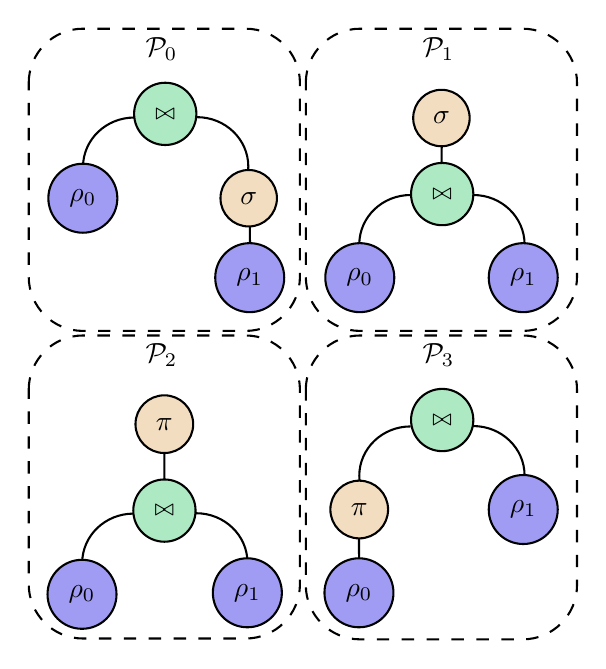
\begin{tikzpicture}[x=0.75pt,y=0.75pt,yscale=-1,xscale=1]
%uncomment if require: \path (0,517); %set diagram left start at 0, and has height of 517

%Rounded Rect [id:dp8624880715884613] 
\draw  [dash pattern={on 4.5pt off 4.5pt}] (105.33,91.13) .. controls (105.33,76.7) and (117.03,65) .. (131.47,65) -- (209.87,65) .. controls (224.3,65) and (236,76.7) .. (236,91.13) -- (236,184.47) .. controls (236,198.9) and (224.3,210.6) .. (209.87,210.6) -- (131.47,210.6) .. controls (117.03,210.6) and (105.33,198.9) .. (105.33,184.47) -- cycle ;
%Shape: Arc [id:dp31494258440043477] 
\draw  [draw opacity=0] (131.49,131.4) .. controls (131.6,118.34) and (142.63,107.79) .. (156.22,107.79) -- (156.22,131.61) -- cycle ; \draw   (131.49,131.4) .. controls (131.6,118.34) and (142.63,107.79) .. (156.22,107.79) ;  
%Shape: Arc [id:dp989525013250071] 
\draw  [draw opacity=0] (186.4,107.61) .. controls (200.06,107.61) and (211.13,118.27) .. (211.13,131.42) .. controls (211.13,133.12) and (210.94,134.78) .. (210.59,136.37) -- (186.4,131.42) -- cycle ; \draw   (186.4,107.61) .. controls (200.06,107.61) and (211.13,118.27) .. (211.13,131.42) .. controls (211.13,133.12) and (210.94,134.78) .. (210.59,136.37) ;  
%Straight Lines [id:da07762631689290767] 
\draw    (211.93,172.72) -- (211.92,159.32) ;
%Rounded Rect [id:dp7394597920421722] 
\draw  [dash pattern={on 4.5pt off 4.5pt}] (238.83,91.13) .. controls (238.83,76.7) and (250.53,65) .. (264.97,65) -- (343.37,65) .. controls (357.8,65) and (369.5,76.7) .. (369.5,91.13) -- (369.5,184.47) .. controls (369.5,198.9) and (357.8,210.6) .. (343.37,210.6) -- (264.97,210.6) .. controls (250.53,210.6) and (238.83,198.9) .. (238.83,184.47) -- cycle ;
%Shape: Arc [id:dp9820020599113808] 
\draw  [draw opacity=0] (264.59,168.74) .. controls (264.7,155.68) and (275.73,145.12) .. (289.32,145.12) -- (289.32,168.94) -- cycle ; \draw   (264.59,168.74) .. controls (264.7,155.68) and (275.73,145.12) .. (289.32,145.12) ;  
%Shape: Arc [id:dp9133069142246233] 
\draw  [draw opacity=0] (319.5,145.12) .. controls (333.16,145.12) and (344.23,155.78) .. (344.23,168.94) -- (319.5,168.94) -- cycle ; \draw   (319.5,145.12) .. controls (333.16,145.12) and (344.23,155.78) .. (344.23,168.94) ;  
%Straight Lines [id:da7184291655448178] 
\draw    (304.18,135.48) -- (304.33,120.53) ;

%Rounded Rect [id:dp7882251059064969] 
\draw  [dash pattern={on 4.5pt off 4.5pt}] (105.33,238.93) .. controls (105.33,224.5) and (117.03,212.8) .. (131.47,212.8) -- (209.87,212.8) .. controls (224.3,212.8) and (236,224.5) .. (236,238.93) -- (236,332.67) .. controls (236,347.1) and (224.3,358.8) .. (209.87,358.8) -- (131.47,358.8) .. controls (117.03,358.8) and (105.33,347.1) .. (105.33,332.67) -- cycle ;
%Shape: Arc [id:dp29183604810464403] 
\draw  [draw opacity=0] (131.09,322.24) .. controls (131.2,309.18) and (142.23,298.62) .. (155.82,298.62) -- (155.82,322.44) -- cycle ; \draw   (131.09,322.24) .. controls (131.2,309.18) and (142.23,298.62) .. (155.82,298.62) ;  
%Shape: Arc [id:dp640450492748722] 
\draw  [draw opacity=0] (186,298.44) .. controls (186,298.44) and (186,298.44) .. (186,298.44) .. controls (199.66,298.44) and (210.73,309.1) .. (210.73,322.26) -- (186,322.26) -- cycle ; \draw   (186,298.44) .. controls (186,298.44) and (186,298.44) .. (186,298.44) .. controls (199.66,298.44) and (210.73,309.1) .. (210.73,322.26) ;  
%Straight Lines [id:da338755697000251] 
\draw    (170.68,282.98) -- (170.67,269.58) ;
%Rounded Rect [id:dp7823365018911086] 
\draw  [dash pattern={on 4.5pt off 4.5pt}] (238.83,238.93) .. controls (238.83,224.5) and (250.53,212.8) .. (264.97,212.8) -- (343.37,212.8) .. controls (357.8,212.8) and (369.5,224.5) .. (369.5,238.93) -- (369.5,333.07) .. controls (369.5,347.5) and (357.8,359.2) .. (343.37,359.2) -- (264.97,359.2) .. controls (250.53,359.2) and (238.83,347.5) .. (238.83,333.07) -- cycle ;
%Shape: Arc [id:dp9169159476965278] 
\draw  [draw opacity=0] (265.25,285.94) .. controls (264.82,284.18) and (264.59,282.33) .. (264.59,280.44) .. controls (264.59,267.28) and (275.66,256.62) .. (289.32,256.62) -- (289.32,280.44) -- cycle ; \draw   (265.25,285.94) .. controls (264.82,284.18) and (264.59,282.33) .. (264.59,280.44) .. controls (264.59,267.28) and (275.66,256.62) .. (289.32,256.62) ;  
%Shape: Arc [id:dp6601308034777329] 
\draw  [draw opacity=0] (319.5,256.44) .. controls (319.5,256.44) and (319.5,256.44) .. (319.5,256.44) .. controls (333.16,256.44) and (344.23,267.1) .. (344.23,280.26) .. controls (344.23,280.73) and (344.21,281.2) .. (344.19,281.66) -- (319.5,280.26) -- cycle ; \draw   (319.5,256.44) .. controls (319.5,256.44) and (319.5,256.44) .. (319.5,256.44) .. controls (333.16,256.44) and (344.23,267.1) .. (344.23,280.26) .. controls (344.23,280.73) and (344.21,281.2) .. (344.19,281.66) ;  
%Straight Lines [id:da8488422162059646] 
\draw    (264.48,321.38) -- (264.47,307.98) ;


% Text Node
\draw (160.17,67.73) node [anchor=north west][inner sep=0.75pt]    {$\mathcal{P}_{0}$};
% Text Node
\draw (293.67,67.73) node [anchor=north west][inner sep=0.75pt]    {$\mathcal{P}_{1}$};
% Text Node
\draw  [fill={rgb, 255:red, 242; green, 221; blue, 192 }  ,fill opacity=1 ]  (304.17, 108.03) circle [x radius= 13.6, y radius= 13.6]   ;
\draw (304.17,108.03) node    {$\sigma $};
% Text Node
\draw  [fill={rgb, 255:red, 173; green, 234; blue, 195 }  ,fill opacity=1 ]  (304.54, 144.67) circle [x radius= 15, y radius= 15]   ;
\draw (304.54,144.67) node  [font=\footnotesize]  {$\bowtie $};
% Text Node
\draw  [fill={rgb, 255:red, 160; green, 156; blue, 243 }  ,fill opacity=1 ]  (264.84, 184.94) circle [x radius= 16.62, y radius= 16.62]   ;
\draw (264.84,184.94) node   [align=left] {$\displaystyle \rho _{0}$};
% Text Node
\draw  [fill={rgb, 255:red, 160; green, 156; blue, 243 }  ,fill opacity=1 ]  (343.59, 184.94) circle [x radius= 16.62, y radius= 16.62]   ;
\draw (343.59,184.94) node   [align=left] {$\displaystyle \rho _{1}$};
% Text Node
\draw  [fill={rgb, 255:red, 173; green, 234; blue, 195 }  ,fill opacity=1 ]  (171.11, 106.03) circle [x radius= 15, y radius= 15]   ;
\draw (171.11,106.03) node  [font=\footnotesize]  {$\bowtie $};
% Text Node
\draw  [fill={rgb, 255:red, 160; green, 156; blue, 243 }  ,fill opacity=1 ]  (131.41, 146.67) circle [x radius= 16.62, y radius= 16.62]   ;
\draw (131.41,146.67) node   [align=left] {$\displaystyle \rho _{0}$};
% Text Node
\draw  [fill={rgb, 255:red, 160; green, 156; blue, 243 }  ,fill opacity=1 ]  (211.81, 184.94) circle [x radius= 16.62, y radius= 16.62]   ;
\draw (211.81,184.94) node   [align=left] {$\displaystyle \rho _{1}$};
% Text Node
\draw  [fill={rgb, 255:red, 242; green, 221; blue, 192 }  ,fill opacity=1 ]  (211.32, 146.67) circle [x radius= 13.6, y radius= 13.6]   ;
\draw (211.32,146.67) node    {$\sigma $};
% Text Node
\draw (160.17,215.23) node [anchor=north west][inner sep=0.75pt]    {$\mathcal{P}_{2}$};
% Text Node
\draw  [fill={rgb, 255:red, 242; green, 221; blue, 192 }  ,fill opacity=1 ]  (170.67, 255.53) circle [x radius= 13.9, y radius= 13.9]   ;
\draw (170.67,255.53) node    {$\pi $};
% Text Node
\draw (293.67,215.23) node [anchor=north west][inner sep=0.75pt]    {$\mathcal{P}_{3}$};
% Text Node
\draw  [fill={rgb, 255:red, 242; green, 221; blue, 192 }  ,fill opacity=1 ]  (264.57, 296.65) circle [x radius= 13.9, y radius= 13.9]   ;
\draw (264.57,296.65) node    {$\pi $};
% Text Node
\draw  [fill={rgb, 255:red, 173; green, 234; blue, 195 }  ,fill opacity=1 ]  (170.71, 297.17) circle [x radius= 15, y radius= 15]   ;
\draw (170.71,297.17) node  [font=\footnotesize]  {$\bowtie $};
% Text Node
\draw  [fill={rgb, 255:red, 173; green, 234; blue, 195 }  ,fill opacity=1 ]  (304.54, 253.53) circle [x radius= 15, y radius= 15]   ;
\draw (304.54,253.53) node  [font=\footnotesize]  {$\bowtie $};
% Text Node
\draw  [fill={rgb, 255:red, 160; green, 156; blue, 243 }  ,fill opacity=1 ]  (131.01, 337.5) circle [x radius= 16.62, y radius= 16.62]   ;
\draw (131.01,337.5) node   [align=left] {$\displaystyle \rho _{0}$};
% Text Node
\draw  [fill={rgb, 255:red, 160; green, 156; blue, 243 }  ,fill opacity=1 ]  (210.67, 336.77) circle [x radius= 16.62, y radius= 16.62]   ;
\draw (210.67,336.77) node   [align=left] {$\displaystyle \rho _{1}$};
% Text Node
\draw  [fill={rgb, 255:red, 160; green, 156; blue, 243 }  ,fill opacity=1 ]  (264.44, 336.77) circle [x radius= 16.62, y radius= 16.62]   ;
\draw (264.44,336.77) node   [align=left] {$\displaystyle \rho _{0}$};
% Text Node
\draw  [fill={rgb, 255:red, 160; green, 156; blue, 243 }  ,fill opacity=1 ]  (343.59, 296.65) circle [x radius= 16.62, y radius= 16.62]   ;
\draw (343.59,296.65) node   [align=left] {$\displaystyle \rho _{1}$};


\end{tikzpicture}

    \caption{4 different query plans $\mathcal{P}_0$, $\mathcal{P}_1$ for query $\mathcal{Q}_0$ and $\mathcal{P}_2$, $\mathcal{P}_3$ for query $\mathcal{Q}_1$. The plans have different ordered instructions, which can save time during single execution or allow for more parallel savings.}
    \label{figure:4_query_plans}
\end{figure}

Figure \ref{figure:4_query_plans} shows the different plans that return the same result. They are structure to best resemble the costs and savings defined in figure \ref{figure:2d_problem_data}. The data defines the combination of $\mathcal{P}_1$ and $\mathcal{P}_2$ to offer the greatest savings. In this case, the step that would warrant such savings would be $\rho_0\bowtie\rho_1$, that is present in both plans. In every other case, there are preliminary operations that distort the result so that it is not shareable by the plans. Nevertheless, one can still share the single steps $\rho_0$ and $\rho_1$, which in this case symbolize the loading of tables into memory. \par

\newpage

\begin{figure}[!h]
    \centering
    \begin{minted}{python}
        ([2, 3, 2],
          [21,  1, 36, 16, 33, 42,  7],
          {(0, 2): -7,
           (0, 3): -13,
           (0, 4): -14,
           (0, 5): -6,
           (0, 6): 0,
           (1, 2): -18,
           (1, 3): -12,
           (1, 4): -17,
           (1, 5): -14,
           (1, 6): -4,
           (2, 5): -5,
           (2, 6): -6,
           (3, 5): -20,
           (3, 6): -12,
           (4, 5): -10,
           (4, 6): 0})
    \end{minted}
    \caption{This is an automatically generated, $n$-dimensional problem. The first array tells us how many plans each query has. This problem has 3 queries, two of which have 2 plans and one with 3 plans. Just like the problem from figure \ref{figure:2d_problem_data}, the second element is an array that contains the cost of each plan, and the third element, which is a dictionary, contains the combinations keys and their respective savings.}
    \label{figure:nd_problem_data}
\end{figure}

The problem space from figure \ref{figure:2d_problem_data} is used for direct comparison between our solution and the solution of Fankhauer et al.\cite{fankhauser_multiple_2021}. As one cannot assume that real life problems will always be limited to 2 queries with 2 problems each, the problem generator enhanced to allow the generation of any number of queries, each of which with their own number of plans, as shown in figure \ref{figure:nd_problem_data}.

\newpage

\subsection{Circuit Design}

The design of the circuit is carefully modelled as to allow easier understanding of its behaviour. Initially, for any $n$ plans, the probabilities of each being the cheapest is unknown, which directly means they are all \emph{equally probable}. To create equal probabilities for all plans, an initial layer consisting of a \emph{Hadamard}-Gate is constructed, as illustrated in figure \ref{figure:4_qubit_circuit_with_h_gates}.

\begin{figure}[!h]
    \centering
    \scalebox{1.0}{
    \Qcircuit @C=1.0em @R=0.2em @!R { \\
	 	\nghost{{\mathcal{P}}_{0} :  } & \lstick{{\mathcal{P}}_{0} :  } \barrier[0em]{3} & \qw & \gate{\mathrm{H}} \barrier[0em]{3} & \qw & \qw & \qw\\
	 	\nghost{{\mathcal{P}}_{1} :  } & \lstick{{\mathcal{P}}_{1} :  } & \qw & \gate{\mathrm{H}} & \qw & \qw & \qw\\
	 	\nghost{{\mathcal{P}}_{2} :  } & \lstick{{\mathcal{P}}_{2} :  } & \qw & \gate{\mathrm{H}} & \qw & \qw & \qw\\
	 	\nghost{{\mathcal{P}}_{3} :  } & \lstick{{\mathcal{P}}_{3} :  } & \qw & \gate{\mathrm{H}} & \qw & \qw & \qw\\
	 	\nghost{} & \lstick{} & \ket{\psi_0} &  & \ket{\psi_1}\\
\\ }}
    \caption{A 4 qubit circuit (here the qubits are not denoted with $q_i$ but $\mathcal{P}_i$, which represent for each plan in the problem) for the problem defined in figure \ref{figure:2d_problem_data} consisting of only \emph{Hadamard}-Gates to create an equal superposition across all plans}
    \label{figure:4_qubit_circuit_with_h_gates}
\end{figure}

\begin{equation}
    \centering
    \begin{split}
        \mathcal{P}_i =\ \ket{0} &=\ \begin{pmatrix}1 \\ 0\end{pmatrix}\\
        \mathrm{H}\mathcal{P}_i =\ \mathrm{H}\ket{0} &=\ \frac{1}{\sqrt{2}}\ket{0} + \frac{1}{\sqrt{2}}\ket{1} =\ \begin{pmatrix}\frac{1}{\sqrt{2}} \\ \frac{1}{\sqrt{2}}\end{pmatrix}\\
    \end{split}
    \label{equation:2d_problem_state_0_1}
\end{equation}

Whereas at state $\ket{\psi_0}$ all qubits are equal to state $\ket{0}$, after the \emph{Hadamard}-Gates at state $\ket{\psi_1}$ they all have the state $\frac{1}{\sqrt{2}}\ket{0} + \frac{1}{\sqrt{2}}\ket{1}$, as shown in equation \ref{equation:2d_problem_state_0_1}. To encode the cost $c_i$ of each plan $\mathcal{P}_i$, the desired behaviour is defined. The goal is to \emph{decrease} the probability of a certain plan being selected if it is expensive. To do this, the parametrizable \emph{RY}-Gate is used on each qubit.

\begin{figure}[!h]
    \centering
    \scalebox{1.0}{
    \Qcircuit @C=1.0em @R=0.2em @!R { \\
	 	\nghost{{q}_{0} :  } & \lstick{{\mathcal{P}}_{0} :  } & \gate{\mathrm{H}} & \gate{\mathrm{R_Y}\,(\mathrm{c_0})} \barrier[0em]{3} & \qw & \qw & \qw\\
	 	\nghost{{q}_{1} :  } & \lstick{{\mathcal{P}}_{1} :  } & \gate{\mathrm{H}} & \gate{\mathrm{R_Y}\,(\mathrm{c_1})} & \qw & \qw & \qw\\
	 	\nghost{{q}_{2} :  } & \lstick{{\mathcal{P}}_{2} :  } & \gate{\mathrm{H}} & \gate{\mathrm{R_Y}\,(\mathrm{c_2})} & \qw & \qw & \qw\\
	 	\nghost{{q}_{3} :  } & \lstick{{\mathcal{P}}_{3} :  } & \gate{\mathrm{H}} & \gate{\mathrm{R_Y}\,(\mathrm{c_3})} & \qw & \qw & \qw\\
	 	\nghost{} : & \lstick{{} } & & & \ket{\psi_2}& \\
    \\ }}
    \caption{The 4 qubit circuit from figure \ref{figure:4_qubit_circuit_with_h_gates} for the problem defined in figure \ref{figure:2d_problem_data} improved with cost encoding \emph{RY}-Gates.}
    \label{figure:4_qubit_circuit_with_h_ry_gates}
\end{figure}

\begin{equation}
    \centering
    \begin{split}
        \mathrm{RY}(c_i)\mathrm{H}\mathcal{P}_i &=\ \begin{pmatrix} \cos{\frac{c_i}{2}} & -\sin{\frac{c_i}{2}} \\ \sin{\frac{c_i}{2}} & \cos{\frac{c_i}{2}} \end{pmatrix}\begin{pmatrix}\frac{1}{\sqrt{2}} \\ \frac{1}{\sqrt{2}}\end{pmatrix}\\
        \mathrm{RY}(c_i)\mathrm{H}\mathcal{P}_i &=\ \frac{1}{\sqrt{2}}\begin{pmatrix}\cos(\frac{c_i}{2}) - \sin(\frac{c_i}{2}) \\ \sin(\frac{c_i}{2}) + \cos(\frac{c_i}{2})\end{pmatrix}\\
    \end{split}
    \label{equation:2d_problem_state_0_1}
\end{equation}


\subsection{Cost Embedding}
\subsection{Savings Embedding}
\subsection{Data}

\newpage
